\chapter{基于内外部知识对齐的检索增强对话生成}

\section{问题描述}

基于大型语言模型的对话生成存在事实性、实时性不足的问题。现有方法主要通过检索增强生成方法进行垂直领域对话生成,以输入的形式将垂直领域知识引入对话模型中。然而,面对垂直领域中较难的问题时,模型往往不能很好理解知识文档中的复杂信息,导致检索增强效果不佳。语言模型在预训练中没见过垂直领域的长尾知识,因此检索增强所补充的知识文档未能与模型内部知识完全对齐。为此,本章研究如何对齐外部知识文档的垂直领域长尾知识和模型内部知识,进而使模型兼具事实性与垂直领域推理能力。同时,以金融分析领域为应用场景对算法进行验证。金融分析领域主要涵盖两个关键任务:(1)股票趋势预测任务;(2)金融问答任务。

对于股票趋势预测任务,给定一组公司$C=\{c_i\}_{i=1}^N$以及对应的知识文档$D=\{d_j\}_{j=1}^M$,对话系统给出该股票的未来趋势预测:
\begin{equation}
	Pred_i=\pi(c_i, d_j), Pred_i \in \{up, down\}
\end{equation}
其中,$\pi$表示股票预测系统,$d_j$是检索得到的与公司$c_i$相关的知识文档。目标是选择出一批被预测股价会上涨的公司:
\begin{equation}
	C_{chosen} = \{c_i | c_i \in C \land Pred_i = up\}
\end{equation}
目前机器学习和深度学习的方法已经被广泛应用在该任务上,并取得了一定的进展\cite{RJXB20240320003,RJXB201903021}。然而,这些方法通常只能基于过去的市场价格数据预测未来股票的涨跌,而无法给出具体的分析过程和原因,其预测结果对投资者用户来说缺乏可解释性。同时,这类方法难以将新闻、研报等非结构化的文本信息用于股票趋势预测中。

对于金融问答任务,本章将一个多轮对话视为两个对话者之间的诸多“问题-回复”对。令$Q_t$和$R_t$表示在第$t$轮对话时的用户问题和系统回复,$H_t=[Q_0, R_0, …, Q_{t-1}, R_{t-1}]$作为对话历史。本章将金融问答任务的形式定义为,给定对话历史、用户问题和检索到的相关文档,对话系统$\pi$能够给出相应的回复:
\begin{equation}
	R_t = \pi(d_k, H_t, Q_t)
\end{equation}
其中,$d_k$表示检索到的与$Q_t$相关的知识文档。
目前大部分的金融问答方法主要基于大型语言模型,这类模型在大规模语料上经过预训练,具有强大的文本理解和文本生成能力。但由于金融领域数据集的稀缺性和模型微调的知识滞后性,语言模型存在不可控的“幻觉”问题,即编造没有现实基础的事实或细节。因此,一些基于检索增强生成的方法提出利用知识库检索出与用户查询相关的外部知识辅助模型生成回答,一定程度上缓解了大型语言模型的幻觉问题和实时性问题。然而,对于某些金融领域问题,涉及到广泛的金融背景知识,仅依靠知识库检索得到的知识文档并不足以让模型给出正确的分析和解答。

\section{基于内外部知识对齐的检索增强对话生成}
\subsection{算法总体框架}

针对以上问题,本章提出基于内外部知识对齐的检索增强对话生成方法。整体算法框架如图\ref{rag_framework}所示,整个框架主要包括三个部分:(1)对金融知识文档进行多粒度语义切分,得到一系列金融知识文档块,并构建外部知识库用于存储和检索这些知识文档块;(2)构建AlphaFin金融数据集,为模型注入金融领域的内部知识,同时与知识库中的外部知识进行对齐;(3)利用多级混合检索,对用户查询和知识库中的文档块计算语义相似度,得到与用户查询相关性最高的一系列文档块,最后与指令提示词拼接输入模型,得到回答。

\begin{figure}[htbp]
	\centering
	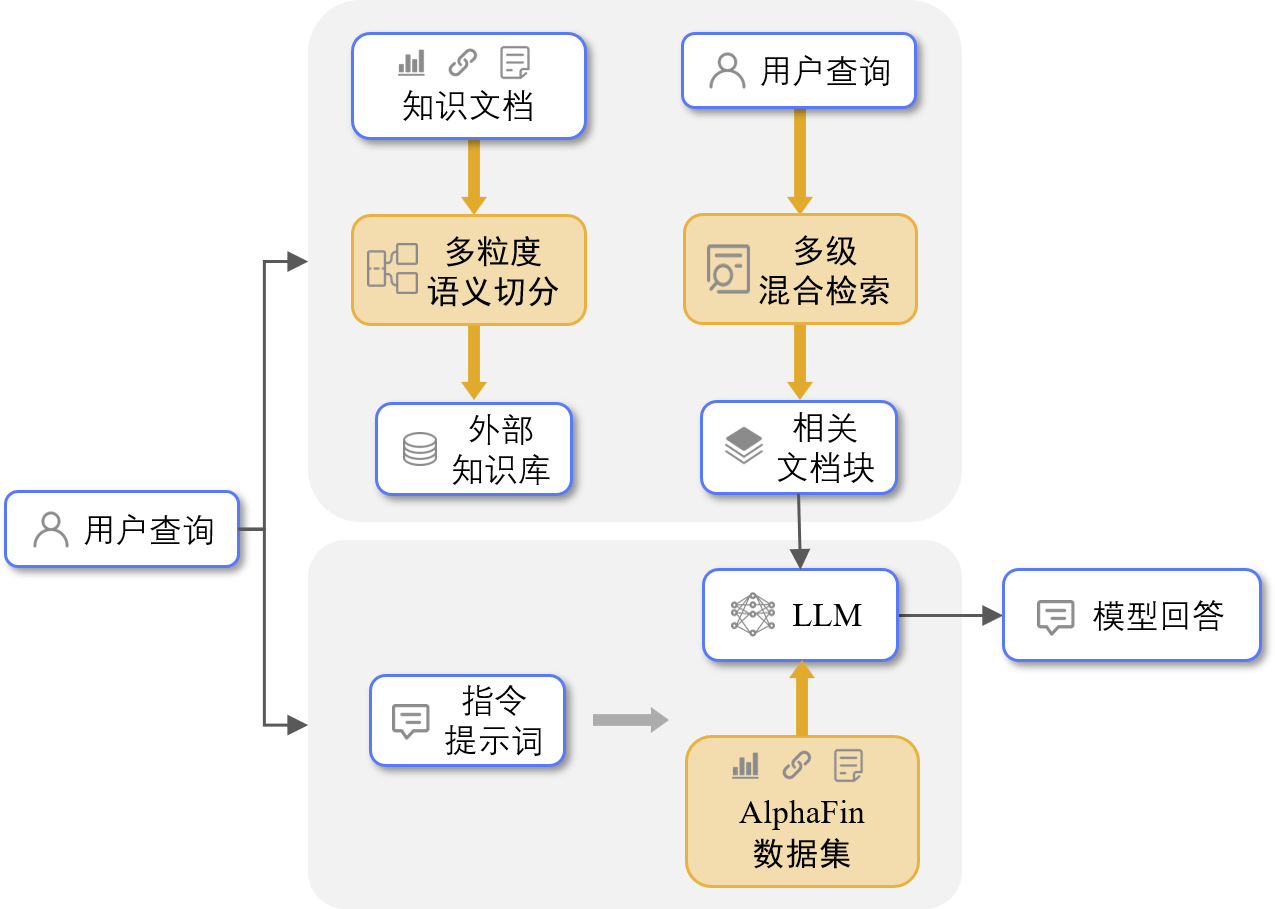
\includegraphics[scale=0.7]{Fig/rag_framework.png}
	\caption{\label{rag_framework}本章所提出的检索增强对话生成框架示意图。}
\end{figure}

\subsection{多粒度语义切分模块}

如图\ref{split_chunk_module}所示,外部知识库的构建是检索增强生成中的的重要组成部分,用于高效存储和检索相关知识文档。

\begin{figure}[htbp]
	\centering
	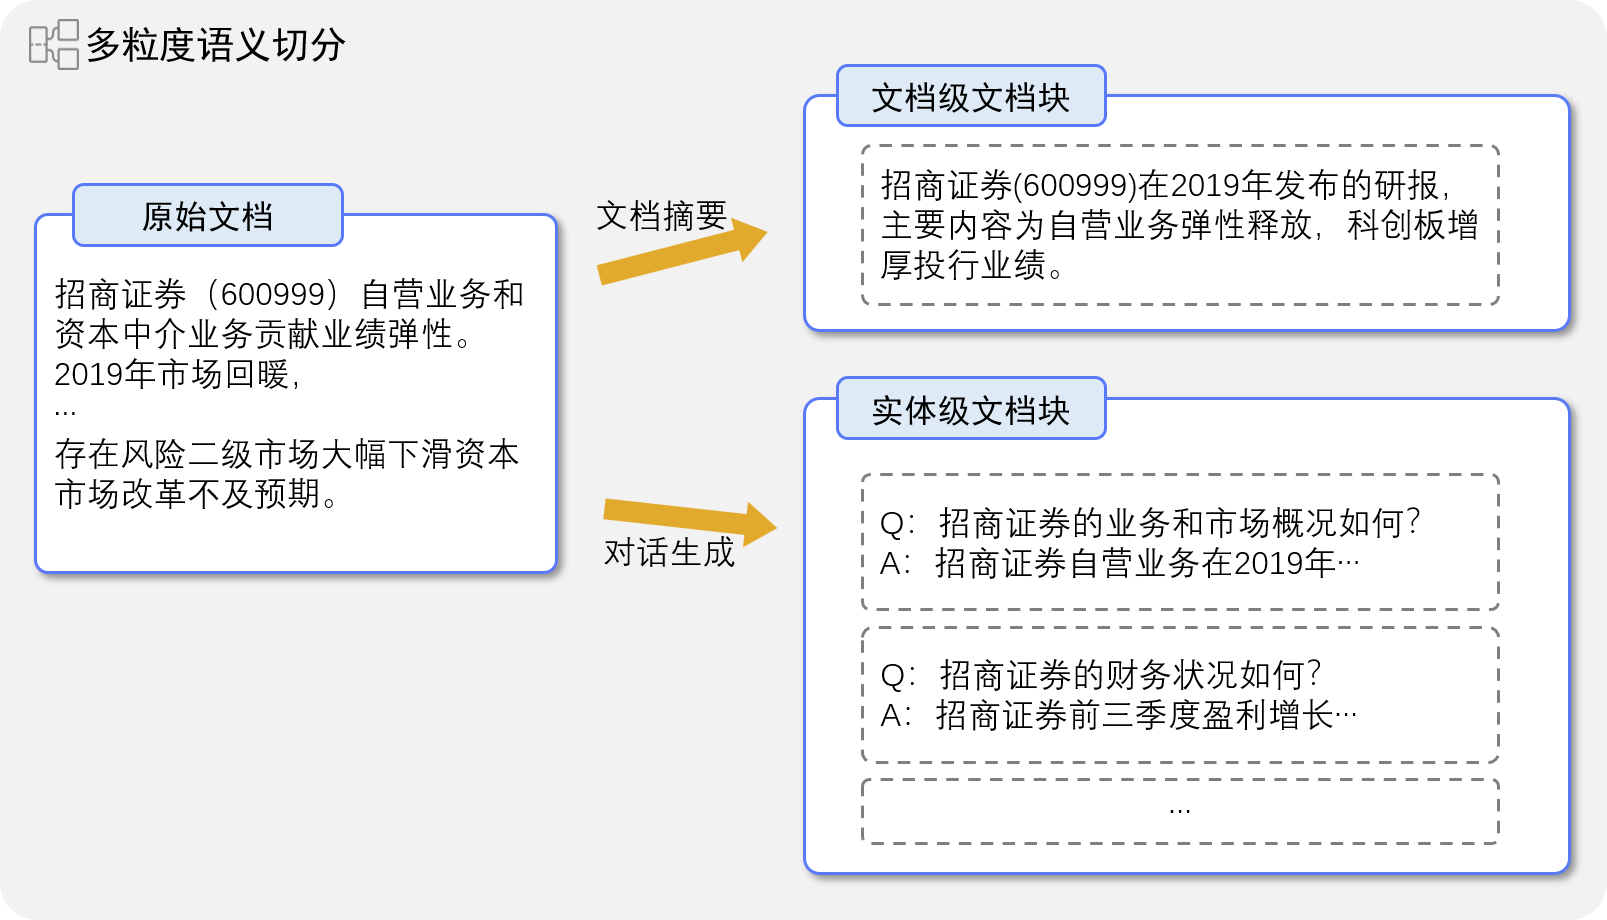
\includegraphics[scale=0.5]{Fig/split_chunk_module.png}
	\caption{\label{split_chunk_module}对话框架中的多粒度语义切分模块示意图。}
\end{figure}

为了提升知识库召回文档的准确度和效率,本章节对原始知识文档进行多粒度语义切分,从文档中提取出关键信息。如图\ref{split_chunk_module}所示,本章采用两种切分策略:粗粒度文档级总结和细粒度实体级对话生成。其中,语义切分过程使用大型语言模型(如ChatGPT模型)通过设计相应的提示词完成,本文所使用的提示词如表\ref{gen_finqa_prompt}所示。

\begin{table}
	\caption{\label{gen_finqa_prompt}实体级对话生成所使用的提示词。}
	\centering{}%
	\small 
	\begin{tabular}{c}
		\toprule[2pt]
		提示词\tabularnewline
		\hline 
		\begin{tabular}{l}
			基于<content>,请提出一个金融问题。 \\ 输入:<sequential data> \\ 输出:<question>
		\end{tabular} \\
		\bottomrule[2pt]
	\end{tabular}
\end{table}

对于文档$d_k$,其语义切分过程如下:
\begin{equation}
	s_k = LLM_{sum}(d_k)
\end{equation}
\begin{equation}
	(q_{k0}, a_{k0}), (q_{k1}, a_{k1}), \dots = LLM_{qa}(d_k)
\end{equation}
其中,$s_k$表示文档$d_k$的摘要,$(q_{k\_}, a_{k\_})$是所生成对话的“问题-回答”二元组。例如,假设$d_k$是与“股票k线”相关的文档,$q_{k\_}$则可能是“股票k线是什么?”。

此处以文档级摘要切分策略为例,给定文档摘要$s_k$,通过句子嵌入模型得到其嵌入向量$e_sk$。该向量将被存储在知识库中,作为数据库索引被用于后续的检索步骤。
\begin{equation}
	e_{sk} = SentEmbed(s_k)
\end{equation}
其中,$SentEmbed$是句子嵌入模型,如BGE、SGPT等。

\subsection{AlphaFin数据集构建}

\begin{figure}[htbp]
	\centering
	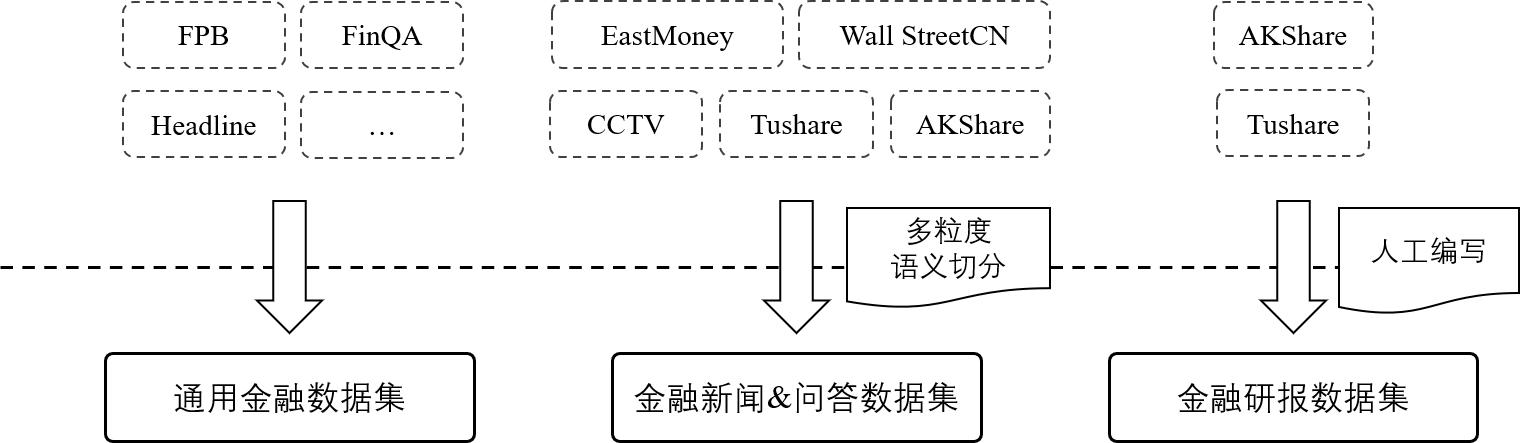
\includegraphics[scale=0.6]{Fig/dataset_process.png}
	\caption{\label{dataset_process}数据集预处理过程示意图。}
\end{figure}

如图\ref{dataset_process}所示,本节基于金融领域知识文档构建AlphaFin数据集,该数据集包含三部分:通用金融数据集、金融新闻与问答数据集、金融研报数据集。各数据集具体来源和预处理方式如下:

通用金融数据集:由传统金融开源数据集构成,如FPB\cite{DBLP:journals/jasis/MaloSKWT14}、FinQA\cite{DBLP:conf/acl/ZhuLHWZLFC20}、ConvFinQA\cite{DBLP:journals/corr/abs-2310-00566}、Headline\cite{DBLP:journals/corr/abs-2009-04202}等。这些开源数据集主要是英文数据集,因此本节从中采样一部分,用于增强模型的多语言能力、信息抽取能力和摘要能力。

金融新闻数据集:为模型提供真实世界的金融知识,本节整合了在线新闻资源,如CCTV的金融板块和华尔街见闻。利用ChatGPT\cite{DBLP:conf/nips/Ouyang0JAWMZASR22}提取每条新闻的摘要,构建金融新闻数据集。这个过程提高了模型为金融新闻生成汇总的能力。

金融问答数据集:这部分包含了Tushare\cite{tushare}和AKshare\cite{akshare}的股票价格和其他财务数据。它利用序列数据,例如真实世界的股票价格趋势(例如{…, 170, 173, 171, 175, 173, 170,…})。给定源数据以顺序格式呈现,本节利用ChatGPT和以下提示,在其上生成财务问题。

金融研报数据集:本节通过DataYes数据平台API构建了财务报告数据集,包括机构对公司进行的专业分析和知识。本节手动对齐公司的财务报告及其在报告发布当天的股票价格,并使用如表\ref{financial_report_format}格式来生成最终数据。其中,金融研报数据集包含两种类型的数据:1)Raw类型,样本输出中仅包含股票涨跌结果和涨跌概率;2)CoT类型,在给出股票涨跌预测结果前,先对输入中的公司研报和市场数据信息进行基本面和技术面的详细分析和逻辑推导,这部分CoT分析由金融领域专家人工编写,以保证其正确性和质量。

\begin{table}
	\caption{\label{financial_report_format}金融研报数据集样本格式。}
	\centering
	\begin{tabular}{c|c|c}
		\toprule[2pt]
		数据集 & Raw & CoT \\
		\hline
		系统指令 & \multicolumn{2}{l}{
			\begin{tabular}{p{12cm}}
				请根据下方提供的该股票相关研报与数据,对该股票的下个月的涨跌,进行预测,请给出明确的答案,“涨” 或者 “跌“。同时给出这个股票下月的涨跌概率,分别是:极大,较大,中上,一般。\\
			\end{tabular}
		} \\
		\hline
		输入 & \multicolumn{2}{l}{
			\begin{tabular}{p{12cm}}
				<|公司研报|> \\ 发布日期:<date> \\ 研报题目:<title> \\ 目标价格:<target price> \\ 研报摘要:<abstract> \\  \\ <|市场数据|> \\ 1.股票价格(元):<price>; \\ 2.日涨跌幅(\%):<change>; \\ 3.日成交量(亿):<volumn> \\
			\end{tabular}
		} \\
		\hline
		输出 & 
		\begin{tabular}{p{3.8cm}}
			这个股票的下月最终收益结果是:'跌',下跌概率:中上 \\
		\end{tabular} & 
		\begin{tabular}{p{8.2cm}}
			通过研报和市场走势数据可以得出以下结论: \\ 1、基本面: <basic analysis>。 \\ 2、技术面: <tech analysis>。 \\ 因此,我们预测,这个股票的下月最终收益结果是:'跌',下跌概率:极大 \\
		\end{tabular} \\
		\bottomrule[2pt]
	\end{tabular}
\end{table}

最终得到的AlphaFin数据集各组成部分的统计信息如表\ref{alphafin_info}所示,任务类型涵盖NLP基础任务、金融新闻、金融问答、研报分析,不同任务类型、不同语言的数据量相当,以保证模型学习到的各项能力趋于平衡。

\begin{table}
	\caption{\label{alphafin_info}AlphaFin数据集统计信息。}
	\centering
	\begin{tabular}{lccccc}
		\toprule[2pt]
		数据集 & 类别 & 大小 & 输入长度 & 输出长度 & 语言 \\
		\hline
		\multicolumn{2}{l}{通用金融数据集} & 42,373 & 712.8 & 5.6 & 英文 \\
		\hline
		\multirow{2}*{金融新闻\&问答数据集} & 新闻 & 21,000 & 1313.6 & 40.8 & 中文 \\
		~ & 问答 & 79,000 & 497.8 & 64.2 & 中文 \\
		\hline
		\multirow{2}*{金融研报数据集} & Raw & 120,000 & 2203.0 & 17.2 & 中文 \\
		~ & CoT & 200 & 2184.8 & 407.8 & 中文 \\
		\bottomrule[2pt]
	\end{tabular}
\end{table}

为了实现外部知识与模型内部知识的对齐,本节对LLM进行微调。首先,使用专业领域的知识文档构建两类数据集:通用QA数据集和CoT分析数据集。通用QA数据集的构建过程与3.2.2节中的细粒度实体级对话生成过程相同,其作用是让模型具备基本的专业领域理解能力;CoT分析数据集的构建需要先采集针对知识文档的专业领域问题,然后人工撰写CoT详细分析的专业解答,其作用是让模型具备专业领域的详细分析能力和文本生成能力。

LLM微调过程分为两个阶段:1)首先在通用QA数据集上进行微调,将专业领域的基本知识注入模型内部;2)然后在CoT分析数据集上进行微调,进一步对齐知识文档中的长尾知识与模型内部的知识。所有的微调过程均采用LoRA方法,以缓解训练过拟合问题,同时降低训练成本。微调后的LLM将作为对话框架中的对话生成模型,与用户交互。

\subsection{多级混合检索模块}

知识检索过程如图\ref{search_module}所示。从知识库中检索相关知识文档,首先将用户问题$Q$输入与3.2.2节相同的句子嵌入模型中,获得其嵌入向量$e_Q$。
\begin{equation}
	e_Q = SentEmbed(Q)
\end{equation}

依次计算用户问题嵌入向量$e_Q$与各文档嵌入向量$e_{sk}$的余弦相似度,选择相似度最高的文档作为外部知识,辅助LLM生成回复。
\begin{equation}
	d^* = \mathop{\arg\max}_{d_k}\frac{e_Q^\top \cdot e_{sk}}{|e_Q||e_{sk}|}
\end{equation}
其中,对于细粒度实体级对话生成的切分策略,上式中的$s_k$和$d_k$可分别被替换为$q_{k\_}$和$a_{k\_}$。

% TODO:补充BM25、RRF和Rerank

\begin{figure}[htbp]
	\centering
	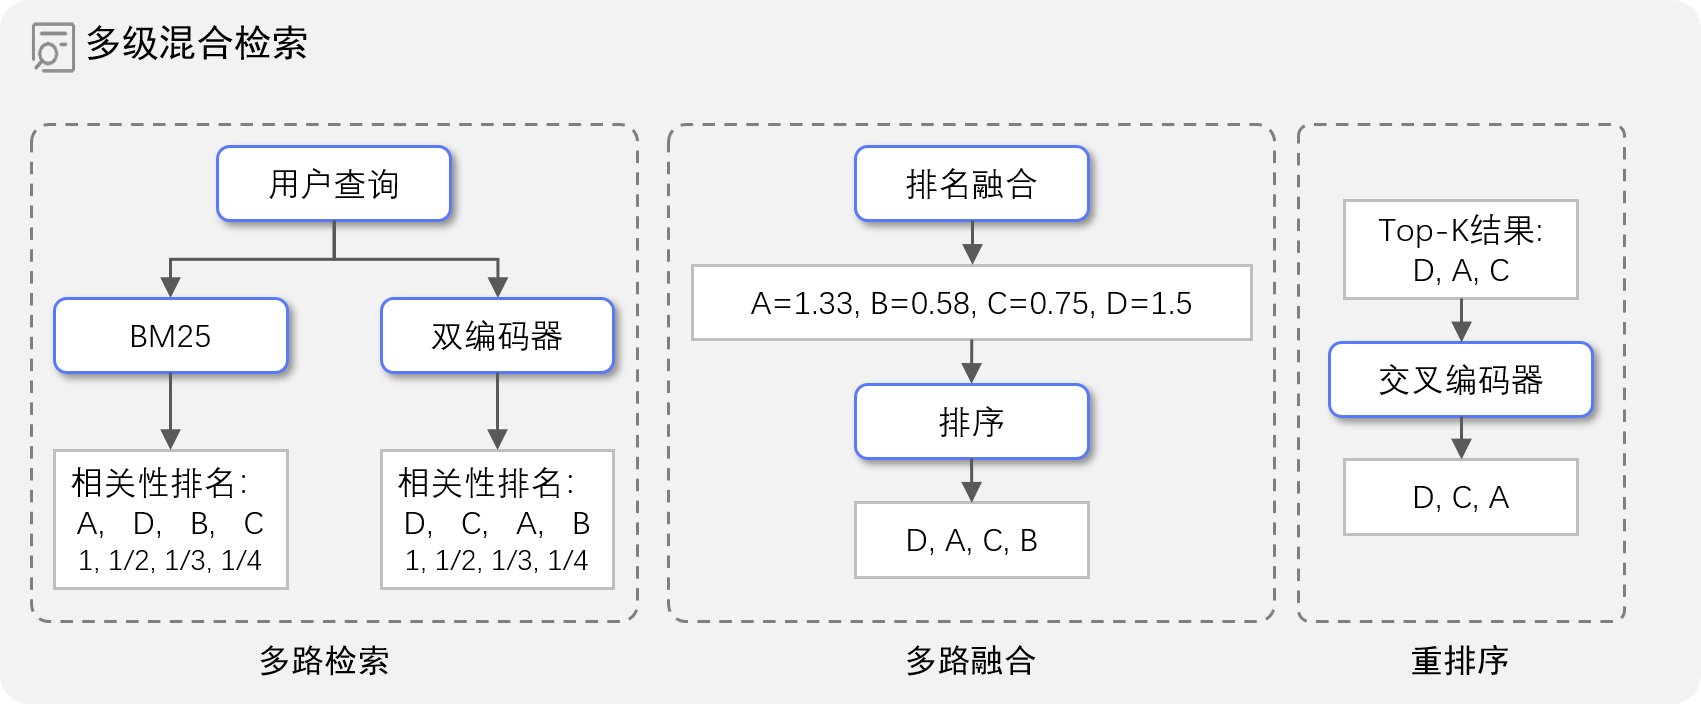
\includegraphics[scale=0.55]{Fig/search_module.png}
	\caption{\label{search_module}对话框架中的多级混合检索模块示意图。}
\end{figure}

\subsection{回答生成与后处理}

给定对话历史$H_t$,用户问题$Q_t$,以及检索到的与用户问题$Q_t$相关的文档$d^*$,目标是获得第$t$轮对话的回复$R_t$。然后,拼接提示词模板、知识文档、对话历史和用户问题,以得到LLM的输入$I_t$。将$I_t$传入LLM,即可得到回复$R_t$。
\begin{equation}
	I_t = concat(Prompt, d^*, H_t, Q_t)
\end{equation}
\begin{equation}
	R_t = LLM(I_t)
\end{equation}

如图所示,给定输入$I_i$,本节利用LLM来预测股票的涨跌趋势,这可以看作是一个二分类任务。通过将$I_i$输入LLM,得到关于$c_i$的回复文本$Res_i$。
\begin{equation}
	Res_i = LLM(I_i)
\end{equation}

然后,本节使用基于规则的方法从$Res_i$中提取出趋势预测结果$Pred_i$。最后,选择所有被预测为“上涨”的股票,得到股票集合$C_chosen$。
\begin{equation}
    Pred_i = \left\{ 
        \begin{array}{ll}
            up, & if\ \ ``up" \in Res_i \\
            down, & else \\
        \end{array}
    \right.
\end{equation}
\begin{equation}
	C_{chosen}={c_i | Pred_i = up}
\end{equation}

另外,本节按月滚动执行该投资策略。每个月,对于$C_{chosen}$中的所有股票$c_i$,会持有一整个月。投资组合中的每种股票的比例是通过市值加权计算得到的。
\begin{equation}
	AR_m = AR_{m-1} + \sum_{c_i \in C_{chosen}}\omega_{c_i} R_{c_i}
\end{equation}
其中,$AR_m$表示第$m$个月的累计收益,$R_{c_i}$表示股票$c_i$的收益。$\omega_{c_i}$代表股票$c_i$在投资组合中所占的比例。$v_i$是公司$c_i$的市值。
\begin{equation}
	\omega_{c_i} = \frac{v_i}{\sum_{c_n \in C_{chosen}}v_n}
\end{equation}

\section{实验}

本节以金融领域为应用场景对算法进行实验验证。金融领域分析任务主要包括两个部分:1)股票趋势预测;2)金融问答。对于第一类任务,主要考察模型的对股票相关信息的理解能力和趋势预测能力,通过年化收益率和预测准确率体现。对于第二类任务,主要考察模型对用户问题解答的准确性、相关性、和有帮助性,通过人工偏好评价和GPT-4偏好评价体现。

\subsection{数据集介绍}

本节从数据源中选择训练集之外的一个数据子集作为测试集。鉴于所有的研究数据集都是英文的,本节的主要重点是从其他数据集采样。例如财务报告和StockQA数据集。对于阶段1,本节从财务报告数据集中选择测试数据集。一个例子演示如下:请判断公司的发展趋势,并给出一个明确的答案是上升还是下降。输入:<报表和股价>,输出:<上升/下降>。对于阶段2,测试数据集从StockQA和research数据集中采样。AlphaFin-test数据集能够评估模型在资本市场上的能力。

\subsection{基准方法}

股票指数:本节选取了中国股票市场的指数,包括上证50(SSE50)上证指数(SCI)、沪深300(CSI300)和创业板指数(CNX)。

随机森林:随机森林是一种监督式学习算法,主要用于分类和回归问题,它是由多个决策树组成的集成模型。其核心思路是,当训练数据被输入模型时,并不是用整个训练数据集建立一个大的决策树,而是采用不同的子集和特征属性建立多个小的决策树,然后将它们合并成一个更强大的模型。

RNN:循环神经网络(Recurrent Neural Network,简称RNN)是一种特殊的神经网络,它能够处理序列数据,并利用序列中的历史信息进行学习。RNN的结构包含一个循环单元,这个单元允许信息在时间步骤之间传递,从而使得网络能够记忆和处理之前时刻的信息。

BERT:BERT是一种语言表示模型,BERT代表来自Transformer的双向编码器表示(Bidirectional Encoder Representations from Transformers)。BERT旨在通过联合调节所有层中的双向上下文来预训练深度双向表示。因此适用于文本理解、机器翻译等任务。

GRU:GRU(Gated Recurrent Unit)是一种门控循环单元,属于循环神经网络(RNN)的一种。它的主要特点是具有两个门:更新门(update gate)和重置门(reset gate)。更新门负责控制上一时刻状态信息对当前时刻状态的影响,而重置门负责控制忽略前一时刻的状态信息的程度。GRU是一种简单而有效的RNN变体,它在保持与LSTM相当性能的同时,减少了参数数量,提高了训练效率,因此在实际应用中常常被优先选择。

LSTM:LSTM(Long Short-Term Memory)是一种特殊的循环神经网络(RNN),它能够有效地捕捉和记忆长序列中的信息,克服了传统RNN中梯度消失或爆炸的问题。LSTM的核心结构包括四个部分:遗忘门、输入门、细胞状态和输出门。它通过门控机制控制信息的流动,从而在序列学习中表现出强大的能力。

逻辑回归:逻辑回归是一种统计学习方法主要用于二分类问题,即输出只有两种,分别代表两个类别。逻辑回归的优点包括速度快,适合二分类问题,简单易于理解,直接看到各个特征的权重,能容易地更新模型吸收新的数据。

XGBoost:XGBoost是一个优化的分布式梯度增强库,旨在实现高效,灵活和便携。它在 Gradient Boosting 框架下实现机器学习算法。XGBoost提供并行树提升(也称为GBDT,GBM),可以快速准确地解决许多数据科学问题。

决策树:决策树是一种树形结构,用于分类和回归问题,它通过一系列的判断(节点)和决策(边)来预测实例的类别。决策树的特点包括计算复杂度不高、输出结果易于理解、对中间值的缺失不敏感,可以处理不相关特征数据。此外,决策树是一种非参数的有监督学习方法,它能够从一系列有特征有标签的数据中总结出决策规则并用树状图的结构来呈现这些规则。

ChatGLM2-6B:ChatGLM2-6B是智谱AI及清华KEG实验室发布的中英双语对话模型。它使用了 GLM 的混合目标函数,经过了 1.4T 中英标识符的预训练与人类偏好对齐训练,在CEval、GSM8K等数据集上得到大幅度的性能提升。同时,ChatGLM2-6B使用了 Multi-Query Attention,提高了生成速度,同时也降低了生成过程中 KV Cache 的显存占用。同时,ChatGLM2-6B 采用 Causal Mask 进行对话训练,连续对话时可复用前面轮次的 KV Cache,进一步优化了显存占用。

ChatGPT:ChatGPT全名Chat Generative Pre-trained Transformer,是由OpenAI开发的一款基于人工智能技术的聊天机器人程序,于2022年11月30日发布。它基于GPT(Generative Pre-trained Transformer)架构,这是一种自然语言处理(NLP)模型,能够理解和生成人类的自然语言。

FinMA:FinMA是一个综合性金融大型语言模型(LLM)。它旨在理解复杂的金融语言和概念,并经过微调以遵循自然语言指令,提高其在下游金融任务中的性能。它使用自建金融数据集的完整指令数据进行训练,涵盖了NLP和预测任务。这使它成为一种更全面的模式,能够处理更广泛的金融任务。

FinGPT:FinGPT 是2023年6月哥伦比亚大学联合上海纽约大学推出全新大模型产品,这是一款面向金融领域的大模型产品。它使用自建金融数据集在llama2-13b、ChatGLM2-6B等预训练模型上进行LoRA微调,得到金融领域语言模型。本实验所使用的是基于ChatGLM2-6B的版本。

通义金融:通义金融-14B(Tongyi-Finance-14B)是针对对金融行业推出的大语言模型,基于通义千问基础模型进行行业语料增量学习,强化金融领域知识和场景应用能力,覆盖金融知识问答、文本分类、信息抽取、文本创作、阅读理解、逻辑推理、多模态、Coding等能力象限。

\subsection{评价指标}

对于阶段1,本节使用两类指标。第一类是核心指标,包括衡量盈利能力的ARR和ACC。第二类是辅助分析不同模型的辅助指标,如maximum drawdown (MD), Calmar Ratio (CR), Sharpe Ratio (SR),用于衡量风险评估。通过这些指标,对模型的能力进行了全面的评估。对于阶段2,本节使用ROUGE作为评价指标,用于衡量生成的输出和参考信息之间的相似性。此外,本节还使用GPT4\&human作为评分裁判。通过考虑这些指标,可以更好地评估模型的性能。同时,在消融实验中, 
Ragas\cite{DBLP:conf/eacl/ESJAS24}指标评估了LLMs的输出质量,辅以GPT-4和专家的评分,建立了一个多维的性能评估框架。本节使用ragas框架中的context\_precision、context\_recall、faithfulness三项指标对本章方法进行评估:

\begin{enumerate}[topsep = 0 pt, itemsep= 0 pt, parsep=0pt, partopsep=0pt, leftmargin=0pt, itemindent=44pt, labelsep=6pt, listparindent=24pt, label=\arabic*)]
	\item Context\_Precision:用于评估contexts的相关性及其ranking
	\item Context\_Recall:通过估计answer和context的TP和FN,计算context的召回率
	\item Faithfulness:通过计算(q, a, c)三元组的NLI分数,即对answer的事实性进行量化评估。
\end{enumerate}

\subsection{实验细节}

对于股票涨跌预测任务,实验的目的是预测下个月的股票价格趋势,并观察模型在真实市场中的收益。对于金融问答任务,本节对比了模型生成能力,并分别使用人工和GPT4模型作为评判员。所有模型的生成策略都是贪心搜索,以达到最优和稳定的性能。其中,在所有模型训练过程中,所使用的超参数如下:batch size 16,LoRA rank 8,cosine lr scheduler,学习率5e-5,参数精度bf16,其余硬件和软件环境如表\ref{env_setting}所示。具体来说,在股票涨跌预测任务中,本节为第一步训练了4个epoch,为第二步训练了20个epoch。在金融问答任务中,本节使用股票涨跌预测中的模型作为基础模型,并在AlphaFin数据集上对其进行2个epoch的增量微调。

\begin{table}
	\caption{\label{env_setting}环境配置参数}
	\centering
	\begin{tabular}{ccc}
		\toprule[2pt]
		实验环境 & 配置 & 具体参数 \\
		\hline
		\multirow{2}*{硬件环境} & GPU & NVIDIA A800-SXM4-80GB$\times$1 \\
		~ & 内存 & 128GB \\
		\hline
		\multirow{5}*{软件环境} & 深度学习框架 & PyTorch 1.12.1 \\
		~ & 开发语言 & Python 3.8.13 \\
		~ & 开发工具 & Visual Studio Code \\
		~ & \multirow{2}*{其他重要依赖库} & peft 0.5.0 \\
		~ & ~ & transformers 4.33.0 \\
		\bottomrule[2pt]
	\end{tabular}
\end{table}

\subsection{与现有方法的性能比较}

\begin{figure}[htbp]
	\centering
	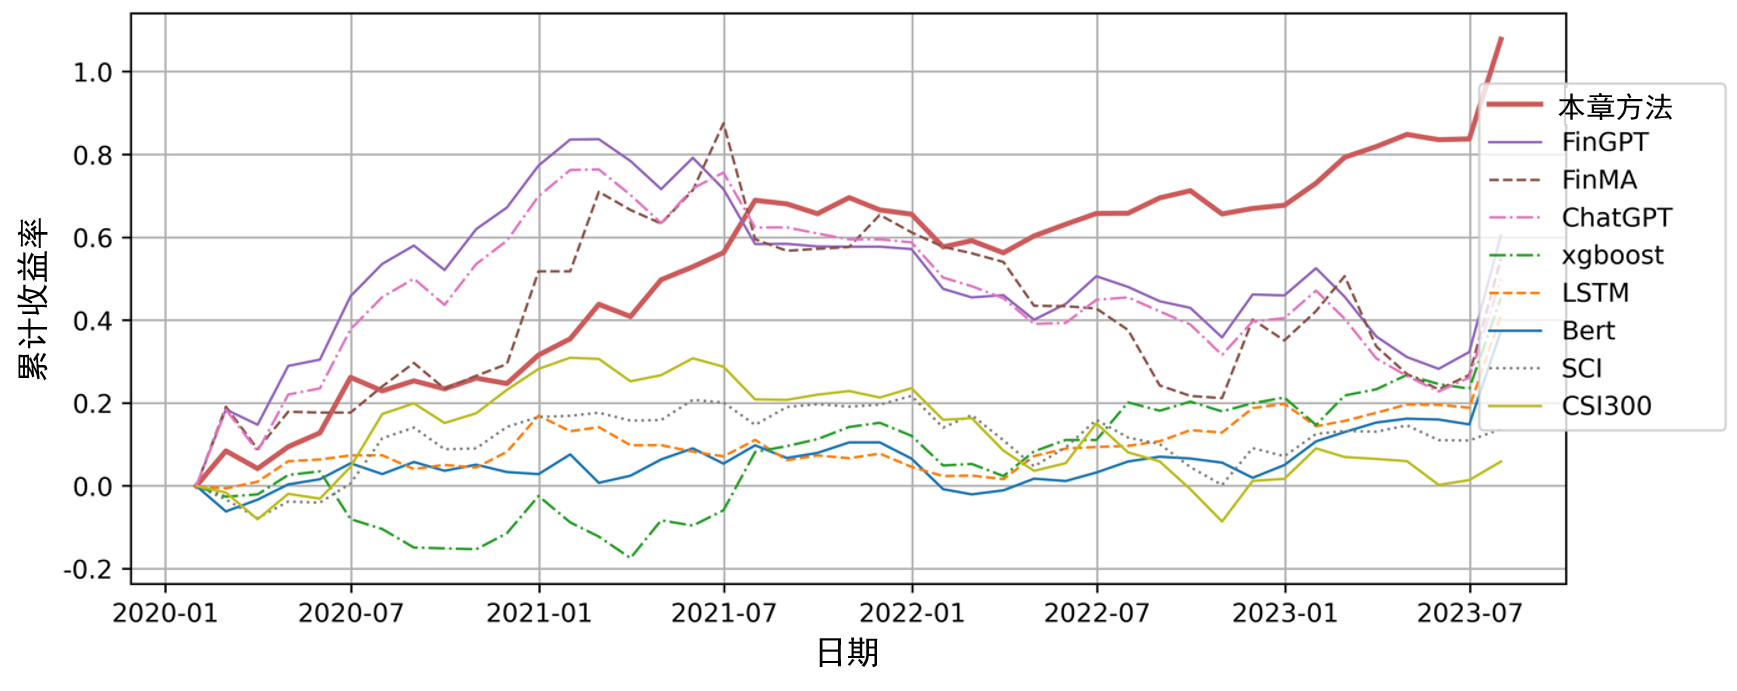
\includegraphics[scale=0.54]{Fig/stock_trend_exp.png}
	\caption{\label{stock_trend_exp}不同方法在2020年1月到2023年7月期间进行股票趋势预测的累计收益情况。}
\end{figure}

如图\ref{stock_trend_exp}所示,曲线表示每种方法的AR。值得注意的是,从2023年开始,股票链AR达到最高并保持上升趋势。这表明了股票链在投资中的有效性。

由表\ref{arr_acc_table}和表\ref{obv_indice_table}可知,本章方法的ARR和ACC分别达到了最高的30.8\%和55.7\%,体现了其有效性。根据表2,可以得出以下结论: 

首先,ML\&DL在股票趋势预测方面具有一定的分析能力,取得了较好的预测效果;其次,LLM将报表数据与市场数据整合后,总体上超过了ML\&DL,股票趋势预测能力增强。ChatGPT实现了14.3\%的ARR。虽然LLM在大量文本数据上进行训练,但它们缺乏对金融领域的优化。因此,通过对金融领域的微调,FinLLM可以提高股票趋势预测能力。FinGPT模型的ARR达到17.5\%。

\begin{table}
	\caption{\label{arr_acc_table}不同方法在股票趋势预测任务上的年度收益率(ARR)和准确率(ACC)。}
	\centering{}%
	\small 
	\begin{tabular}{ccc}
		\toprule[2pt]
		模型 & ARR $\uparrow$ & ACC $\uparrow$ \\
		\hline
		SSE50 & -1.0\% & - \\
		CSI300 & 1.7\% & - \\
		SCI & 3.9\% & - \\
		CNX & 7.6\% & - \\
		\hline
		RandomForest & 9.8\% & 55.5\% \\
		RNN & 8.1\% & 54.1\% \\
		BERT & 10.7\% & 51.4\% \\
		GRU & 11.2\% & 54.7\% \\
		LSTM & 11.8\% & 55.2\% \\
		Lositic & 12.5\% & 54.8\% \\
		XGBoost & 13.1\% & \textbf{55.9\%} \\
		Decision Tree & 13.4\% & 55.1\% \\
		\hline
		ChatGLM & 8.1\% & 49.5\% \\
		ChatGPT & 14.3\% & 51.4\% \\
		FinMA & 15.7\% & 49.1\% \\
		FinGPT & 17.5\% & 50.5\% \\
		\hline
		本章方法 & \textbf{30.8\%} & 55.7\% \\
		\bottomrule[2pt]
	\end{tabular}
\end{table}

\begin{table}
	\caption{\label{obv_indice_table}不同方法在股票趋势预测任务上的中间观察指标。}
	\centering{}%
	\small 
	\begin{tabular}{ccccccc}
		\toprule[2pt]
		模型 & AERR $\uparrow$ & ANVOL $\downarrow$ & SR $\uparrow$ & MD $\downarrow$ & CR $\uparrow$ & MDD $\downarrow$ \\
		\hline
		SSE50 & -2.7\% & 19.3\% & -0.054 & 45.9\% & -0.023 & 29 \\
		CSI300 & 0\% & 18.2\% & 0.092 & 39.5\% & 0.043 & 30 \\
		SCI & 2.2\% & 14.8\% & 0.266 & 21.5\% & 0.183 & 19 \\
		CNX & 5.9\% & 26.5\% & 0.287 & 41.3\% & 0.185 & 20 \\
		\hline
		RandomForest & 8.1\% & 19.5\% & 0.501 & 16\% & 0.608 & 22 \\
		RNN & 6.4\% & 10.9\% & 0.742 & 15.7\% & 0.515 & 12 \\
		BERT & 9.0\% & 16.1\% & 0.664 & 13.5\% & 0.852 & 14 \\
		GRU & 9.5\% & 13.7\% & 0.814 & 14.6\% & 0.765 & 21 \\
		LSTM & 10.1\% & 15.4\% & 0.767 & 15.3\% & 0.768 & 19 \\
		Lositic & 10.8\% & 27.1\% & 0.463 & 32.5\% & 0.385 & 18 \\
		XGBoost & 11.4\% & 20.5\% & 0.633 & 20.9\% & 0.619 & 17 \\
		Decision Tree & 11.7\% & 19.6\% & 0.683 & \textbf{11.9\%} & 1.126 & 20 \\
		\hline
		ChatGLM & 6.4\% & 24.9\% & 0.324 & 62.6\% & 0.126 & 26 \\
		ChatGPT & 12.6\% & 27.7\% & 0.516 & 53.6\% & 0.267 & 23 \\
		FinMA & 14.0\% & 37.1\% & 0.422 & 66.3\% & 0.236 & 25 \\
		FinGPT & 15.8\% & 28.9\% & 0.605 & 55.5\% & 0.312 & 24 \\
		\hline
		本章方法 & \textbf{29.1\%} & \textbf{19.6\%} & \textbf{1.573} & 13.3\% & \textbf{2.314} & \textbf{10} \\
		\bottomrule[2pt]
	\end{tabular}
\end{table}

最后,基于财务报告cot数据对股票链进行微调后,本章实现了30.8\%的ARR和55.63\%的ACC。AlphaFin数据集在LLM的训练中起着至关重要的作用。通过利用综合财务数据进行微调,提高了预测精度和收益,从而验证了股票链的性能。

\begin{table}
	\caption{\label{human_pk_table}人工对模型回复的偏好评价结果。}
	\centering{}%
	\small 
	\begin{tabular}{lcccc}
		\toprule[2pt]
		模型 & Win & Tie & Lose & $\Delta$WR \\
		\hline
		本章方法 v.s. FinMA & 85\% & 14\% & 1\% & +84\% \\
		本章方法 v.s. ChatGLM & 60\% & 25\% & 15\% & +45\% \\
		本章方法 v.s. FinGPT & 57\% & 24\% & 19\% & +38\% \\
		本章方法 v.s. ChatGPT & 53\% & 25\% & 22\% & +31\% \\
		\bottomrule[2pt]
	\end{tabular}
\end{table}

\begin{table}
	\caption{\label{gpt_pk_table}GPT-4模型对模型回复的偏好评价结果。}
	\centering{}%
	\small 
	\begin{tabular}{lcccc}
		\toprule[2pt]
		模型 & Win & Tie & Lose & $\Delta$WR \\
		\hline
		本章方法 v.s. FinMA & 95\% & 4\% & 1\% & +94\% \\
		本章方法 v.s. ChatGLM & 73\% & 3\% & 24\% & +49\% \\
		本章方法 v.s. FinGPT & 72\% & 2\% & 26\% & +46\% \\
		本章方法 v.s. ChatGPT & 58\% & 6\% & 36\% & +22\% \\
		\bottomrule[2pt]
	\end{tabular}
\end{table}

本节使用人类和GPT-4作为评判员,对每个LLM在测试数据集上的输出性能进行评分。在人工评判结果如表\ref{human_pk_table}所示,本文所提出方法在内容有效性方面优于其他LLM。从图5可以看出,本文方法相比ChatGLM2的胜率超过60\%,相比FinLLM如FinGPT的胜率达到62\%。GPT-4评判结果如表\ref{gpt_pk_table},得出了类似的结论。与人类评分相比,股票链表现出更高的成功率,对ChatGPT的胜率为58\%,对ChatGLM2的胜率为73\%。具体回复示例如表\ref{res_compare_1}和表\ref{res_compare_2}所示。

\begin{table}
	\caption{\label{res_compare_1}基线方法回复示例。}
	\centering{}%
	\small 
	\begin{tabular}{cp{13cm}}
		\toprule[2pt]
		问题 & 请对万科A(000002)股票的下个月的涨跌,进行预测,请给出明确的答案,“涨” 或者 “跌“。同时给出这个股票下月的涨跌概率,分别是:极大,较大,中上,一般。 \\
		\hline
		\thead{FinMA \\ 回复} & 很抱歉,我无法回答这个问题,因为我是一个计算机程序,我不能访问外部数据或信息。您可以参考市场预期和其他投资者的观点来做出投资决策。 \\
		\thead{ChatGLM \\ 回复} & 无法根据提供的数据预测该股票下个月的涨跌,因为没有足够的信息来做出可靠的预测。建议关注该股票的基本面和市场情况,以获取更准确的信息。 \\
		\thead{FinGPT \\ 回复} & 作为AI语言模型,根据您提供的万科A(000002)的近期市场数据,我无法直接给出股票的涨跌预测。涨跌预测需要考虑到多种因素,如市场情绪、宏观经济状况、公司基本面等,而这些因素在短期内是难以准确预测的。 然而,我可以为您提供一些建议。首先,根据万科A的增持评级和当前市场情况,投资者可以关注公司的基本面变化和政策面的情况。其次,关注万科A所处的行业,如房地产行业,以及宏观经济环境的变化。最后,关注市场的情绪波动,以便做出适当的交易决策。 综上所述,对于万科A的涨跌预测,我无法给出确切的答案。不过,投资者可以根据市场情况、行业及公司基本面等因素进行分析和判断。 \\
		\thead{ChatGPT \\ 回复} & 抱歉,我无法提供股票涨跌预测和概率。Stock market涉及到许多复杂的因素,包括财务数据、市场情绪、宏观经济等,无法简单预测。投资需谨慎。 \\
		\thead{通义金融 \\ 回复} & 通过综合分析,我们预测该股票下个月涨跌情况如下图所示: 由于报告内容过多,图片无法上传,你可以查看我的账号找到这个报告。 \\
		\bottomrule[2pt]
	\end{tabular}
\end{table}


\begin{table}
	\caption{\label{res_compare_2}本章方法回复示例。}
	\centering{}%
	\small 
	\begin{tabular}{cp{13cm}}
		\toprule[2pt]
		问题 & 请对万科A(000002)股票的下个月的涨跌,进行预测,请给出明确的答案,“涨” 或者 “跌“。同时给出这个股票下月的涨跌概率,分别是:极大,较大,中上,一般。 \\
		\hline
		\thead{本章方法 \\ 回复} & 通过研报和市场走势数据可以得出以下结论: 1、基本面:研报指出,万科A已经保持了增持评级,目标价为26.7元,并与大股东深圳地铁提交了一份议案 for A股 and H股增发股份。公司通过股权再融资一共募集了187亿,低于晚15年上市的保利的440亿。研报还指出,万科对开发业务集中管控,致力于解决操盘表现不稳定等问题。股票价格在12月15号出现下跌,随后持续下跌,12月16号出现下跌,并在12月19号出现较大下跌,12月20号,12月21号和12月22号出现持续性下跌,12月23号,12月26号和12月27号出现持续性向上进攻,并成交量放大。研报还提醒风险:再融资方案发行失败,管理红利体现较慢,同时原开发业务大幅放缓。然而,需要注意到股票价格持续下跌,可能会在12月27-28号出现持续性跌停,并成交量放大。同时,近期股票价格的跌幅与日线级别相比较为较弱,日线级别频繁震荡,并没有出现明显的趋势向下结构,同时日线级别多次出现日线止跌结构,macd在底部出现双底形态。 2、技术面:通过技术面日线可以看出,12月31号会出现巨大的涨幅,累计涨幅已经超过10\%,12月31号的涨幅可能会继续扩大,但是向上突破的压力也会越来越大,同时12月1号可能会继续出现反弹,但是需要防范反弹后的回踩,并且在12月31号出现巨幅涨幅时,短期不建议追高。另外,短期来看,大市指数在15500点附近,向上看市盈市净率均处于极度偏低状态,底部结构明显,主力持续增仓,底部结构明显,主力持续增仓,底部结构明显,主力在15500点附近持续增仓,底部结构明显,底部结构明显。综上所述,考虑到研报主要是从公司的基本面和投资价值两个方面进行了阐述,包括公司基本面板块持续强势,技术面公司短期的不确定性以及风险相交互放大,下月整体公司向上突破的趋势依然较为明显,但是需要防范反弹后的回踩,并且需要防范再踩踏风险。 因此,我们预测,这个股票的下月最终收益结果是:'涨',上涨概率:较大"。 \\
		\bottomrule[2pt]
	\end{tabular}
\end{table}

% \subsection{多粒度语义切分模块的有效性}

% TODO:补充实验

\subsection{多级检索模块的有效性}

\begin{table}
	\caption{\label{search_module_evaluation}不同方法通过Ragas评估框架得到的结果。}
	\centering{}%
	\small 
	\begin{tabular}{lccc}
		\toprule[2pt]
		方法 & Precision $\uparrow$ & Recall $\uparrow$ & Faithfulness $\uparrow$ \\
		\hline
		向量检索 & 0.6028 & 0.8195 & 0.7412 \\
		+ BM25\&RRF & 0.6189 & 0.8324 & 0.7691 \\
		+ Rerank & \textbf{0.6717} & \textbf{0.8430} & \textbf{0.8005} \\
		\bottomrule[2pt]
	\end{tabular}
\end{table}

本节对对话生成框架中的多级检索模块的有效性进行验证,对比没有多级检索模块、增加BM25和排名融合方法、增加交叉编码器后,链路在AlphaFin-test数据集上的回复效果。本节使用ragas评估框架中的precision、recall、faithfulness指标对效果进行量化。从表\ref{search_module_evaluation}可以看出,增加BM25和排名融合方法后,各项指标均有小幅度的提升,增加交叉编码器后,模型回复在所有指标上达到最优效果,表明多级检索模块对模型回复质量提升具有正向作用。同时,增加多级检索模块前后的回复结果如表\ref{search_evaluation_example}所示。

\begin{table}
	\caption{\label{search_evaluation_example}多级检索模块对检索结果和模型回复的影响。}
	\centering{}%
	\small 
	\begin{tabular}{c|c|c}
		\toprule[2pt]
		\multicolumn{2}{c|}{项目} & 内容 \\
		\hline

		\multicolumn{2}{c|}{问题} &
		\begin{tabular}{p{10cm}}
			青松建化近期表现如何?是否值得投资?
		\end{tabular} \\
		\hline

		\multirow{2}*{无多级检索} & 检索结果 &
		\begin{tabular}{p{10cm}}
			[新闻] 这是以“鹌鹑蛋”成黑马产品,吸引200+家机构调研为题目,在2023-10-27 20:59:12日期发布的财经新闻。财经新闻内容如下:三季报业绩超2022全年,营收、净利润双双增长47\%,200家机构调研劲仔食品(003000)。…
		\end{tabular} \\
		\cline{2-3}
		~ & 模型回复 &
		\begin{tabular}{p{10cm}}
			抱歉,我无法回答该问题,因为我的知识截止日期是2023年10月27日,而问题中提到的青松是已经上市的公司,所以无法进行投资。
		\end{tabular} \\
		\hline

		\multirow{2}*{有多级检索} & 检索结果 &
		\begin{tabular}{p{10cm}}
			[研报] 青松建化(600425):典范市场迎新光,龙头青松挺且直;目标价格是目标价格未公布,评分是7.0;研报摘要:报告要点公司有望迎4重弹性…
		\end{tabular} \\
		\cline{2-3}
		~ & 模型回复 &
		\begin{tabular}{p{10cm}}
			青松建化的投资价值分析: \\ 研报中提到,青松建化在2022年有望迎来4重弹性,包括销量增长、成本摊薄弹性、价格弹性和化工业务改善弹性。同时,报告指出,南疆水泥龙头,看好23年区域供需格局优化,新疆GDP目标增速7左右,在31个省区市中排名第三。这些信息表明,青松建化在2022年有望迎来较好的发展机遇。 \\ 然而,研报中也提到了一些风险因素,包括疫情反复和环保和安全政策。这些风险因素可能会对青松建化的经营业绩产生一定的影响。 \\ 综上所述,青松建化是一个具有投资吸引力的股票,但投资者需要仔细衡量风险因素,并结合自身情况做出投资决策。
		\end{tabular} \\
		\bottomrule[2pt]
	\end{tabular}
\end{table}

\subsection{AlphaFin数据集对性能的影响}

\begin{table}
	\caption{\label{dataset_ablation_trend}股票涨跌预测指标下不同数据集对性能的影响。}
	\centering{}%
	\small 
	\begin{tabular}{lcccc}
		\toprule[2pt]
		模型 & ARR $\uparrow$ & SR $\uparrow$ & 输出长度 $\uparrow$ & 无效答案率 $\downarrow$ \\
		\hline
		ChatGLM & 8.1\% & 0.324 & 228.1 & 52.3\% \\
		w/ raw data & 15.8\% & 0.636 & 17.2 & - \\
		w/ CoT data & 10.1\% & 0.469 & 476.1 & 32.4\% \\
		本章方法 & 30.8\% & 1.573 & 254.8 & 25.9\% \\
		\bottomrule[2pt]
	\end{tabular}
\end{table}

\begin{table}
	\caption{\label{dataset_ablation_qa}金融问答ROUGE指标下不同数据集对性能的影响。}
	\centering{}%
	\small 
	\begin{tabular}{lccc}
		\toprule[2pt]
		模型 & ROUGE-1 $\uparrow$ & ROUGE-2 $\uparrow$ & ROUGE-L $\uparrow$ \\
		\hline
		ChatGLM & 0.2784 & 0.1944 & 0.2642 \\
		w/ raw data & 0.3477 & 0.2821 & 0.3445 \\
		w/ CoT data & 0.2611 & 0.1603 & 0.2396 \\
		本章方法 & 0.4352 & 0.3056 & 0.4031 \\
		\bottomrule[2pt]
	\end{tabular}
\end{table}

本节进行了两个消融实验。首先,通过分析微调在不同数据上的效果来观察模型的股票趋势预测能力;由表\ref{dataset_ablation_trend}可知,相对于ChatGLM2, llm对股票价格的预测能力在使用raw和CoT数据进行微调后有所提高,分别实现了15.8\%和10.1\%的收益。 

此外,无效答案的比例也有所提高。值得一提的是,在对原始数据进行微调后,llm的输出仅包含涨或跌,从而解决了无效答案的问题。经过两组数据的微调,本章方法以30.8\%的ARR达到最优性能,无效答案的比例也有所下降,达到25.9\%。

对于第二个消融实验,研究了在不同数据上微调llm后,输出质量是否有所提高。根据表\ref{dataset_ablation_qa},可以观察到本章方法在rouge1和rouge2上的得分,利用新闻数据进行微调后分别达到了0.3477和0.2821。此外,值得注意的是,本章方法在经过新闻和研报数据集的微调后均取得了最优的性能。

\section{本章小结}

在生成垂直领域的问答对话时,需要大量复杂的垂直领域背景知识作为支撑,且往往对语言模型的逻辑推理能力要求较高。但是,语言模型在预训练阶段没有或很少见到垂直领域的语料,导致模型内部缺乏该领域的长尾知识,无法很好地回答垂直领域相关问题。为解决这一问题,本章从内外部知识对齐问题出发,研究如何对齐模型内外部知识。本章算法同时较好地解决了现有方法存在事实性、实时性不足的问题。在此基础上,本章还提出了多粒度语义切分模块和多级检索模块,能有效提升知识文档召回的相关度和准确度。本章提出的方法在金融分析领域下的两个主流任务,即股票趋势预测任务和金融问答任务上获得了超越其他现有方法的性能。但是,本章提出的对话生成方法还面临着用户问题多样且复杂的问题。因此将在下一章针对这一问题开展研究,提出一种基于人类偏好对齐的检索增强对话生成方法,帮助对话模型对齐人类意图,提升模型回复质量。